\section{Aktuelles Korrelationsformat zur Modifikation von Artefaktmetadaten}\label{sec:current-correlation-format}

Das Korrelationsformat wurde 2021 entwickelt, um manuelle Nachkorrekturen an den durch die \enquote{CPE Derivation} automatisch abgeleiteten \acrshort{cpe}-Identifikatoren zu ermöglichen.
Während der Hauptanwendungsfall daraus besteht, fehlerhafte oder unpassende \acrshort{cpe}-Zuordnungen zu korrigieren, ermöglicht es die Modifikation beliebiger Artefaktattribute, und wurde so über die Zeit für viele weitere Anwendungsfälle eingesetzt.

Das Format basiert auf \acrfull{yaml} und folgt einem zweistufigen Modell:
Über einen Selektor werden Regeln für die Auswahl von Artefakten definiert, und dann eine Reihe an Modifikationen, die an diesem Artefakt vorgenommen werden sollen.
Jeder Korrelationseintrag kann aus den folgenden Attributen bestehen, wobei mindestens ein \texttt{affects} und eine Modifikationsoperation definiert sein muss.
Ein kleines Beispiel bei dem eine \acrshort{cpe} zu einem Artefakt hinzugefügt wird kann in \autoref{lst:correlation-initial-example} gefunden werden, ausführlichere Beispiele mit Beschreibungen werden nach der Formatbeschreibung aufgeführt.

\begin{lstlisting}[style=yaml,caption={Korrelationseintrag für die Java-Komponente Liquibase},label={lst:correlation-initial-example}]
- affects:
    - Id: liquibase-*.jar
    - Id: org.liquibase.liquibase-*.jar
  append:
    Additional CPE URIs: cpe:/a:liquibase:liquibase
\end{lstlisting}

\paragraph{Artefakt-Selektion}
Die \texttt{affects}-Sektion eines Eintrages muss immer vorhanden sein und legt fest, auf welche Artefakte sich der Eintrag beziehen soll.
Dabei wird in einer Listenstruktur eine Menge an Attribut-Wert-Paaren angegeben, die auf der Ebene der Liste logisch als ODER-Verknüpfung interpretiert werden und die Attribute innerhalb der Liste mit einer UND-Verknüpfung verbunden sind.
Das bedeutet, dass bereits ein zutreffendes Listenelement ausreicht, um einen Treffer zu erzielen, aber innerhalb jedes Elements müssen alle angegebenen Attribut-Werte-Paare auf das zu prüfende Artefakt zutreffen.
Die betroffenen Attribute können beliebige Felder aus einem Artefakt sein (etwa \texttt{Id}, \texttt{Component}, \texttt{Group Id}, \texttt{Type}, \ldots).
Es ist dadurch möglich domänenübergreifende Selektionskriterien zu formulieren.

Optional kann ein \texttt{ignores}-Block definiert werden, der vom Aufbau her der \texttt{affects}-Sektion entspricht, aber die Logik umkehrt.
Sobald einer der Listeneinträge mit einem Artefakt erfolgreich verglichen wurde, wird das Artefakt von dem Eintrag ausgeschlossen.
Damit können Ausnahmen und Abgrenzungen zu ähnlichen Artefakten erstellt werden, etwa bei Artefakten mit ähnlichen Namen aber unterschiedlichen Ökosystemen.

Die zu vergleichenden Werte der Attribut-Wert-Paare unterstützen mehrere Matching-Modi.
Im einfachsten Fall wird ein Text auf Gleichheit mit dem Attributinhalt verglichen, hierzu wird der Text einfach aufgeführt.
In diesem einfachen Vergleichsmodus können Platzhalterzeichen verwendet werden, so steht ein Sternchen (\texttt{*}) für beliebig viele Zeichen und ein Fragezeichen (\texttt{?}) für ein einzelnes beliebiges Zeichen.
Über zwei Stufen können sich die Werte regulären Ausdrücken annähern:
Ähnlich zu der Notation wie sie in JavaScript verwendet wird \autocite{MdnRegularExpressions2025} können durch das Anhängen von einem Schrägstrich und einer Menge an Flags wie in \enquote{\texttt{/i}} beispielsweise auch case-insensitive Vergleiche durchführen, ohne vollständig auf reguläre Ausdrücke zu wechseln.
Die vollständige Nutzung von regulären Ausdrücken wird ermöglicht, wenn das Muster von vorne und hinten durch \enquote{\texttt{/}} eingerahmt wird.
Durch diese inkrementelle Syntax kann einfach zwischen unterschiedlichen Matching-Modi gewählt werden.

\paragraph{Artefakt-Modifikation}
Sobald ein Artefakt durch einen Eintrag als betroffen erkannt wird, werden die im zweiten Teil des \acrshort{yaml}-Blocks definierten Modifikationen angewandt.
Auch hier gibt es unterschiedliche Weisen, die Attribute der Artefakte zu modifizieren, wobei sich das allgemeine Schema bei den meisten gleicht:
Jede Art an Modifikation führt eine Menge an Attributen, die jeweils einen Text-Wert zugeordnet haben.
Die am häufigsten verwendete Operation ist \texttt{append}, die auf \acrfull{csv}-Attributen angewendet wird, und den angegeben Wert entweder mit einem Komma getrennt an den vorhandenen angehängt wird, oder direkt gesetzt wenn noch keiner vorhanden ist.
Typischerweise betrifft dies \acrshortpl{cpe}, die nachträglich als gültig oder unpassend erkannt wurden und zu einer entsprechenden Liste hinzugefügt werden sollen.
Ähnlich operiert \texttt{remove}, womit auch hier der auf dem Artefakt vorhandene Wert und der im Korrelationseintrag angegebene Wert als \acrshort{csv}-Werte interpretiert und an Kommas getrennt werden und die Schnittmenge der beiden Listen vom Artefakt-Attribut entfernt werden.
\enquote{overwrite} ersetzt den kompletten Inhalt eines Attributs mit einem neuen Werte und \enquote{clear} entfernt ein Attribut von einem Artefakt.

\bigskip

Mit diesen Methoden, auf Artefakte zuzugreifen, können potenziell alle Transformationen an Artefakten durchgeführt werden, die von Interesse sind.
Im Kontext der \acrshort{cpe}-Zuordnung sind besonders die drei Felder relevant, die auch schon in \autoref{subsec:effective-cpe-calculation} aufgeführt wurden:
\texttt{Additional CPE URIs}, \texttt{Inapplicable CPE URIs} und \texttt{CPE URIs}.

Ein Konsens, der sich über die Zeit aus Gründen der Nachvollziehbarkeit geformt hat, ist das Hinzufügen eines Kommentarblocks vor dem Korrelationseintrag mit Informationen über das Artefakt, für den der Eintrag angelegt wurde und eine Begründung, warum er nötig ist.
Dieser Kommentar kann beliebige Begründungen enthalten, etwa Verweise auf Dokumentationen, URLs zu Projektseiten oder kurze Erklärungen, warum etwa eine bestimmte \acrshort{cpe} als passend oder unpassend eingestuft wurde.
Bei späteren Revisionen und Diskussionen im Team erleichtert das die Nachvollziehbarkeit vergangener Entscheidungen.

\paragraph{Inkrementelle Korrelationseinträge}\label{par:incremental-correlation-entries}
werden ermöglicht, da für ein Artefakt alle Korrelationseinträge im Datensatz ausgewertet werden und nicht einfach bei einem ersten zutreffenden gestoppt wird.
Dadurch können aufeinanderfolgende Korrelationseinträge definiert werden, die nacheinander auf ein Artefakt angewendet werden, um einen gewünschten Effekt zu erzielen.

Ein beispielhafter Anwendungsfall betrifft Artefakte mit dem Namensbestandteil \enquote{git} (vgl. \autoref{lst:correlation-incremental-git-example}).
Oft wird auf Artefakten die \acrshort{cpe} \texttt{cpe:/a:github:github} durch die CPE URI Derivation automatisch hinzugefügt, die den Text-Schnipsel \texttt{git} in ihrem Namen enthalten.
Oft wird durch die automatische \acrshort{cpe} URI Derivation die \acrshort{cpe} \texttt{cpe:/a:github:github} zugewiesen, die den GitHub Enterprise Server\footnote{\url{https://docs.github.com/en/enterprise-server/admin/all-releases}} referenziert.
Um es für den Großteil der Einträge im \acrshort{yaml}-Format einfacher zu machen, deaktiviert ein generischer Eintrag diese \acrshort{cpe} für alle Artefakte, die \enquote{git} in egal welchem Attribut enthalten.
Ein spezifischer Folgeeintrag darunter führt die tatsächliche \texttt{git}-Kommandozeilenapplikation auf, bei der dann die falsche \texttt{cpe:/a:github:github} nicht mehr behandelt werden muss, sondern nur noch die konkreten git-spezifischen \acrshortpl{cpe} aufgeführt werden können.
Ein weiterer Eintrag könnte in dem Fall, dass tatsächlich der Enterprise Server gemeint ist, die entsprechende \acrshort{cpe} wieder hinzufügen.

So können allgemeine Muster an einer Stelle behandelt werden und artefaktspezifische Regeln ohne diese isoliert aufgeführt werden können.
Diese Trennung verhindert Redundanzen und vereinfacht spätere Anpassungen.
In \autoref{fig:correlation-utilities-demo} können oben rechts weitere Beispiele dieser allgemeinen Einträge gefunden werden.

\begin{lstlisting}[style=yaml,caption={Inkrementelle Korrelationseinträge für das Kommandozeilentool git},label={lst:correlation-incremental-git-example}]
- affects:
    - any: "*git*/i"
  append:
    Inapplicable CPE URIs: cpe:/a:github:github

- affects:
    - Component: git
      Type: package
  append:
    Inapplicable CPE URIs: cpe:/a:codesys:git, cpe:/a:cygwin:git, cpe:/a:git:git-shell, cpe:/a:gitforwindows:git, cpe:/a:jenkins:git
    Additional CPE URIs: cpe:/a:git:git, cpe:/a:git-scm:git, cpe:/a:git_project:git
\end{lstlisting}

\subsection{Beispiele zu Korrelationsdaten}

\paragraph{Beispiel 1: snappy-1.1.8}
In \autoref{lst:correlation-snappy} ist ein Beispiel aufgeführt, bei dem ein Artefakt \texttt{snappy-1.1.8} als ein Linux Package (Typ \texttt{package}) in einem Softwareinventar identifiziert wurde.
Der CPE URI Derivation-Algorithmus hat in das Attribut \texttt{Derived CPE URIs} seine Identifikation aufgenommen, nämlich \texttt{cpe:/a:knplabs:snappy}.
Vom Namen her sieht diese Identifikation vielleicht überzeugend aus, allerdings stellt sich dies als eine Fehlidentifikation heraus, denn die \acrshort{cpe} verlinkt in ihren Metadaten auf \url{https://github.com/KnpLabs/snappy}, was eine PHP Bibliothek ist und kein Linux Paket.
Erst bei einer manuellen Suche kommt eine zweite \acrshort{cpe} hervor, \texttt{cpe:/a:google:snappy}, die tatsächlich ein Linux Paket darstellt welches nicht nur vom Namen her passt, sondern auch von der Versionsreichweite der veröffentlichten Versionen.
Allerdings wurde auch eine Java-Bibliothek mit demselben Namen identifiziert, also mussten die entsprechenden jar-Dateien über \texttt{ignores} ausgeschlossen werden.
Alternativ hätte auch das \texttt{affects} mit \texttt{Type: package} erweitert werden können, um die Artefakte so zu limitieren.
So ergibt sich der gesamte Eintrag, in dem allgemein alle mit \texttt{snappy-} startenden Artefakte ausgewählt werden, die mit \texttt{.jar} hinten exkludiert und auf den Restlichen die jeweiligen \acrshortpl{cpe} als anwendbar oder nicht in die Artefakt-Attribute mit aufgenommen werden.
In der Praxis würde nun noch ein weiterer Eintrag für die PHP-Bibliothek angelegt werden, der auf den korrekten \texttt{Type} prüft.

\begin{lstlisting}[style=yaml,caption={Korrelationseintrag für Snappy-Komponenten},label={lst:correlation-snappy}]
# Id: snappy-1.1.8
# Component: snappy
# Version: 1.1.8
# Type: package
# Derived CPE URIs: cpe:/a:knplabs:snappy
# reason:
#   cpe:/a:knplabs:snappy --> https://github.com/KnpLabs/snappy --> "PHP library allowing thumbnail, snapshot or PDF generation from a url or a html page." --> PHP library
#   cpe:/a:google:snappy --> https://github.com/google/snappy --> https://pkgs.alpinelinux.org/package/edge/main/x86/snappy --> linux package --> matches this package version range
#   ignore https://mvnrepository.com/artifact/org.xerial.snappy/snappy-java
- affects:
    - Id: snappy-*
  ignores:
    - Id: snappy-*.jar
  append:
    Inapplicable CPE URIs: cpe:/a:knplabs:snappy
    Additional CPE URIs: cpe:/a:google:snappy
\end{lstlisting}

\paragraph{Beispiel 2: Microsoft Windows 10 (Version 21H2)}
Auch nicht-\acrshort{cpe}-Attribute können auf Artefakten ergänzt werden.
In dem Beispiel in \autoref{lst:correlation-win-10-21H2} wird eine Microsoft-Produkt-Id zu dem Betriebssystem Windows 10 in der Version 21H2 zugeordnet.
Der \href{https://github.com/org-metaeffekt/metaeffekt-documentation/blob/bd184b2889d5421b5a71dcd26c1ac0ffc63d07e7/metaeffekt-vulnerability-management/data-mirror/msrc/understanding-data.md}{Dokumentationeintrag zu den Microsoft-Datenquellen} und in \autoref{subsec:msrc-product-ids} wird das Microsoft-Produktidentifikator-Ökosystem näher erklärt, aber prinzipiell haben alle versionierten Produkte in der Microsoft-Datenbank eine eindeutige numerische Id, unter der Schwachstellen registriert werden.
Daher muss nur auf die exakten Attribute geprüft werden und dann kann die korrekte Produkt-Id zu dem Artefakt hinzugefügt werden.
Zusätzlich wird für das EOL-Ökosystem die entsprechende Produkt-Id \texttt{windows} hinzugefügt und eine für die Abfrage spezifische Version die in diesem Ökosystem verwendet werden muss.

\begin{lstlisting}[style=yaml,caption={Korrelationseintrag für Windows 10},label={lst:correlation-win-10-21H2}]
# reason: https://learn.microsoft.com/de-de/windows/release-health/release-information
#   11931 --> Version 21H2 (OS build 19044) / Windows 10 Version 21H2 for x64-based Systems
- affects:
    - Id: Microsoft Windows 10*
      Version: 10.0.19044*
      Type: operating system
      Architecture: "*64*"
    - Id: Windows 10*
      Version: 10.0.19044*
      Type: operating system
      Architecture: "*64*"
  append:
    MS Product ID: "11931"
    EOL Id: windows
    EOL Overwrite Cycle Query Version: 10 21H2 (E)
\end{lstlisting}

\subsection{Automatisch generierte Korrelationsdaten}\label{subsec:old-generated-correlation-data}

Bereits im aktuellen Korrelationssystem hat sich die Notwendigkeit ergeben, gewisse Datenquellen zur automatisierten Generierung von Korrelationseinträgen zu verwenden.
Dieser Prozess wird im Moment manuell ausgelöst, und muss dementsprechend regelmäßig durchgeführt werden.
Im Moment wird hier nur das \acrshort{cpe} Dictionary der \acrshort{nvd} verwendet, um Versionen, Paketnamen und URLs zu gewissen \acrshort{cpe} auszulesen.
Das Dictionary wird im Moment auf zwei Ökosysteme angewandt, die im Folgenden vorgestellt werden.

\paragraph{Java JRE/JDK}
Es hat sich herausgestellt, dass die unterschiedlichen JRE/JDK-Versionen nicht nur unterschiedliche \acrshortpl{cpe} zugewiesen bekommen, sondern auch als eine der wenigen \acrshort{cpe} das \texttt{update}-Feld für ihre Updates innerhalb der Versionen verwenden.
Die Erfassung des Update-Wertes aus dem Versions-Attribut der Artefakte ist für die Systeme der \metaeffektsp herausfordernd, darum hat man sich entschlossen, die bekannten Versionen mit ihren Updates aus dem \acrshort{cpe} Dictionary auszulesen.
Jedes JRE/JDK hat seine eigenen Versionsformate, darum ist es erforderlich diesen Prozess beliebig konfigurierbar zu machen.
Daraus ist ein einfaches Generatorformat in JSON entstanden, das für jede angegebene Version in einer \acrshort{cpe} einen Eintrag generiert, den er nach einer Schablone auffüllt.
Die produktiv eingesetzte Generatordatei kann in \autoref{ch:generatorformat-jre-jdk} zur Referenz gefunden werden.

In \autoref{lst:correlation-generated-zulu-example} kann eine der generierten Dateien für das Zulu JDK gesehen werden:
Es wird ein allgemeiner Eintrag ganz oben ohne Versionsangaben (beliebige Version) generiert, und darunter für jede bekannte Version und jedes Update.

\begin{lstlisting}[style=yaml,caption={Automatisch generierte Korrelationseinträge zu Zulu JDK},label={lst:correlation-generated-zulu-example}]
- affects:
  - Id: /zulu.*-(?:jre|jdk)-headless-.*/i
  - Id: /zulu.*-(?:jre|jdk)-.*/i
  append:
    Additional CPE URIs: cpe:/a:azul:zulu
- affects:
  - Id: /zulu.*-(?:jre|jdk)-headless-11\.0\.10.*/i
  - Id: /zulu.*-(?:jre|jdk)-11\.0\.10.*/i
  append:
    CPE URIs: cpe:/a:azul:zulu:11.0.10
- affects:
  - Id: /zulu.*-(?:jre|jdk)-headless-1\.8\.0.*[^0-9]282.*/i
  - Id: /zulu.*-(?:jre|jdk)-1\.8\.0.*[^0-9]282.*/i
  append:
    CPE URIs: cpe:/a:azul:zulu:8:update282
\end{lstlisting}

\paragraph{NPM-Pakete}

Das \acrshort{cpe} Dictionary enthält eine Vielzahl an Einträgen, die in ihren Referenzen URLs auf die Plattform \texttt{npmjs.com} enthalten.
Diese Metadaten werden ausgelesen, um automatisch die \acrshortpl{cpe} zu finden, die zu NPM-Paketen gehören.
Für jeden dieser Einträge wird dann geprüft, ob aus der URL ein Paketname für reguläre oder \enquote{scoped} NPM-Pakete extrahiert werden kann.
Für diejenigen, bei denen diese Extraktion erfolgreich war, werden aus diesem Namen verschiedene Repräsentationen abgeleitet, wie sie im Dateisystem vorkommen könnten, um unterschiedliche mögliche Namensvarianten des Pakets zu unterstützten.

Mit diesen Namen werden anschließend Korrelationseinträge zwischen zugehörigen Artefakten und \acrshortpl{cpe} generiert.
Um die Nachvollziehbarkeit zu erhöhen, werden die referenzierten URLs bei den Einträgen in dem Kommentarfeld mit aufgenommen.
Das Ergebnis ist eine automatisch generierte Datei mit YAML-Einträgen, ein beispielhafter Eintrag ist in \autoref{lst:correlation-generated-walletconnect-example} dargestellt.

\begin{lstlisting}[style=yaml,caption={Automatisch generierte Korrelationseinträge zu react-walletconnect},label={lst:correlation-generated-walletconnect-example}]
# reason: https://www.npmjs.com/package/@web3-react/walletconnect
#         https://uniswap.org/
- affects:
    - Component: "web3-react_walletconnect"
      Type: /(web|nodejs|npm)-module/
    - Component: "walletconnect"
      Type: /(web|nodejs|npm)-module/
    - Component: "@web3-react/walletconnect"
      Type: /(web|nodejs|npm)-module/
  append:
    Additional CPE URIs: cpe:/a:uniswap:web3-react_walletconnect
\end{lstlisting}

\subsection{Correlation Utilities als Tool zur Korrelationsarbeit}\label{subsec:correlation-utilities}

Die \enquote{Correlation Utilities} sind ein spezialisiertes Experten-Werkzeug zur Analyse von Software-Inventaren im Rahmen der Erstellung und Pflege von Korrelationsdaten.
Ein Software-Inventar mit dem Ziel der korrekten Schwachstellenzuordnung manuell durchzuarbeiten ist ein komplexer und zeitintensiver Prozess.
Die Correlation Utilities stellen eine dedizierte Benutzeroberfläche dar, mit der die spezifischen Aufgabenbereiche dieser Arbeit unterstützt werden.

Technisch besteht das Werkzeug aus einer Spring-Boot-basierten Backend-Anwendung und einem Frontend, das über kachelartige Widgets dynamisch vom Nutzer angeordnet werden kann.
Eine typische Sitzung beginnt mit der Auswahl eines Inventars und dem automatisierten Anreichern von Schwachstellinformationen und begibt sich dann auf den Prozess, jedes Artefakt in dem Inventar auf seine \acrshort{cpe}-Zuordnungen einzeln zu prüfen und Korrekturen durch das Anlegen von neuen Korrelationseinträgen vorzunehmen.

In \autoref{fig:correlation-utilities-demo} kann eine beispielhaft angeordnete Nutzeroberfläche gesehen werden.
Die Benutzeroberfläche in dieser Anordnung besteht links oben aus der Tabelle der Artefakte, mit farbigen Status-Indikatoren pro Zeile um schnell nach relevanten Metriken filtern zu können.
Links unten ist ein Widget zu sehen, das eine Detailsicht mit allen Attributen des aktuell ausgewählten Artefakts anzeigt.
Hier werden zudem über Web-Requests und lokale Datenbankabfragen diverse weitere Informationen, Links und Internetsuchen aggregiert und für den Nutzer vorbereitet.

\begin{figure}
    \centering
    \makebox[\linewidth]{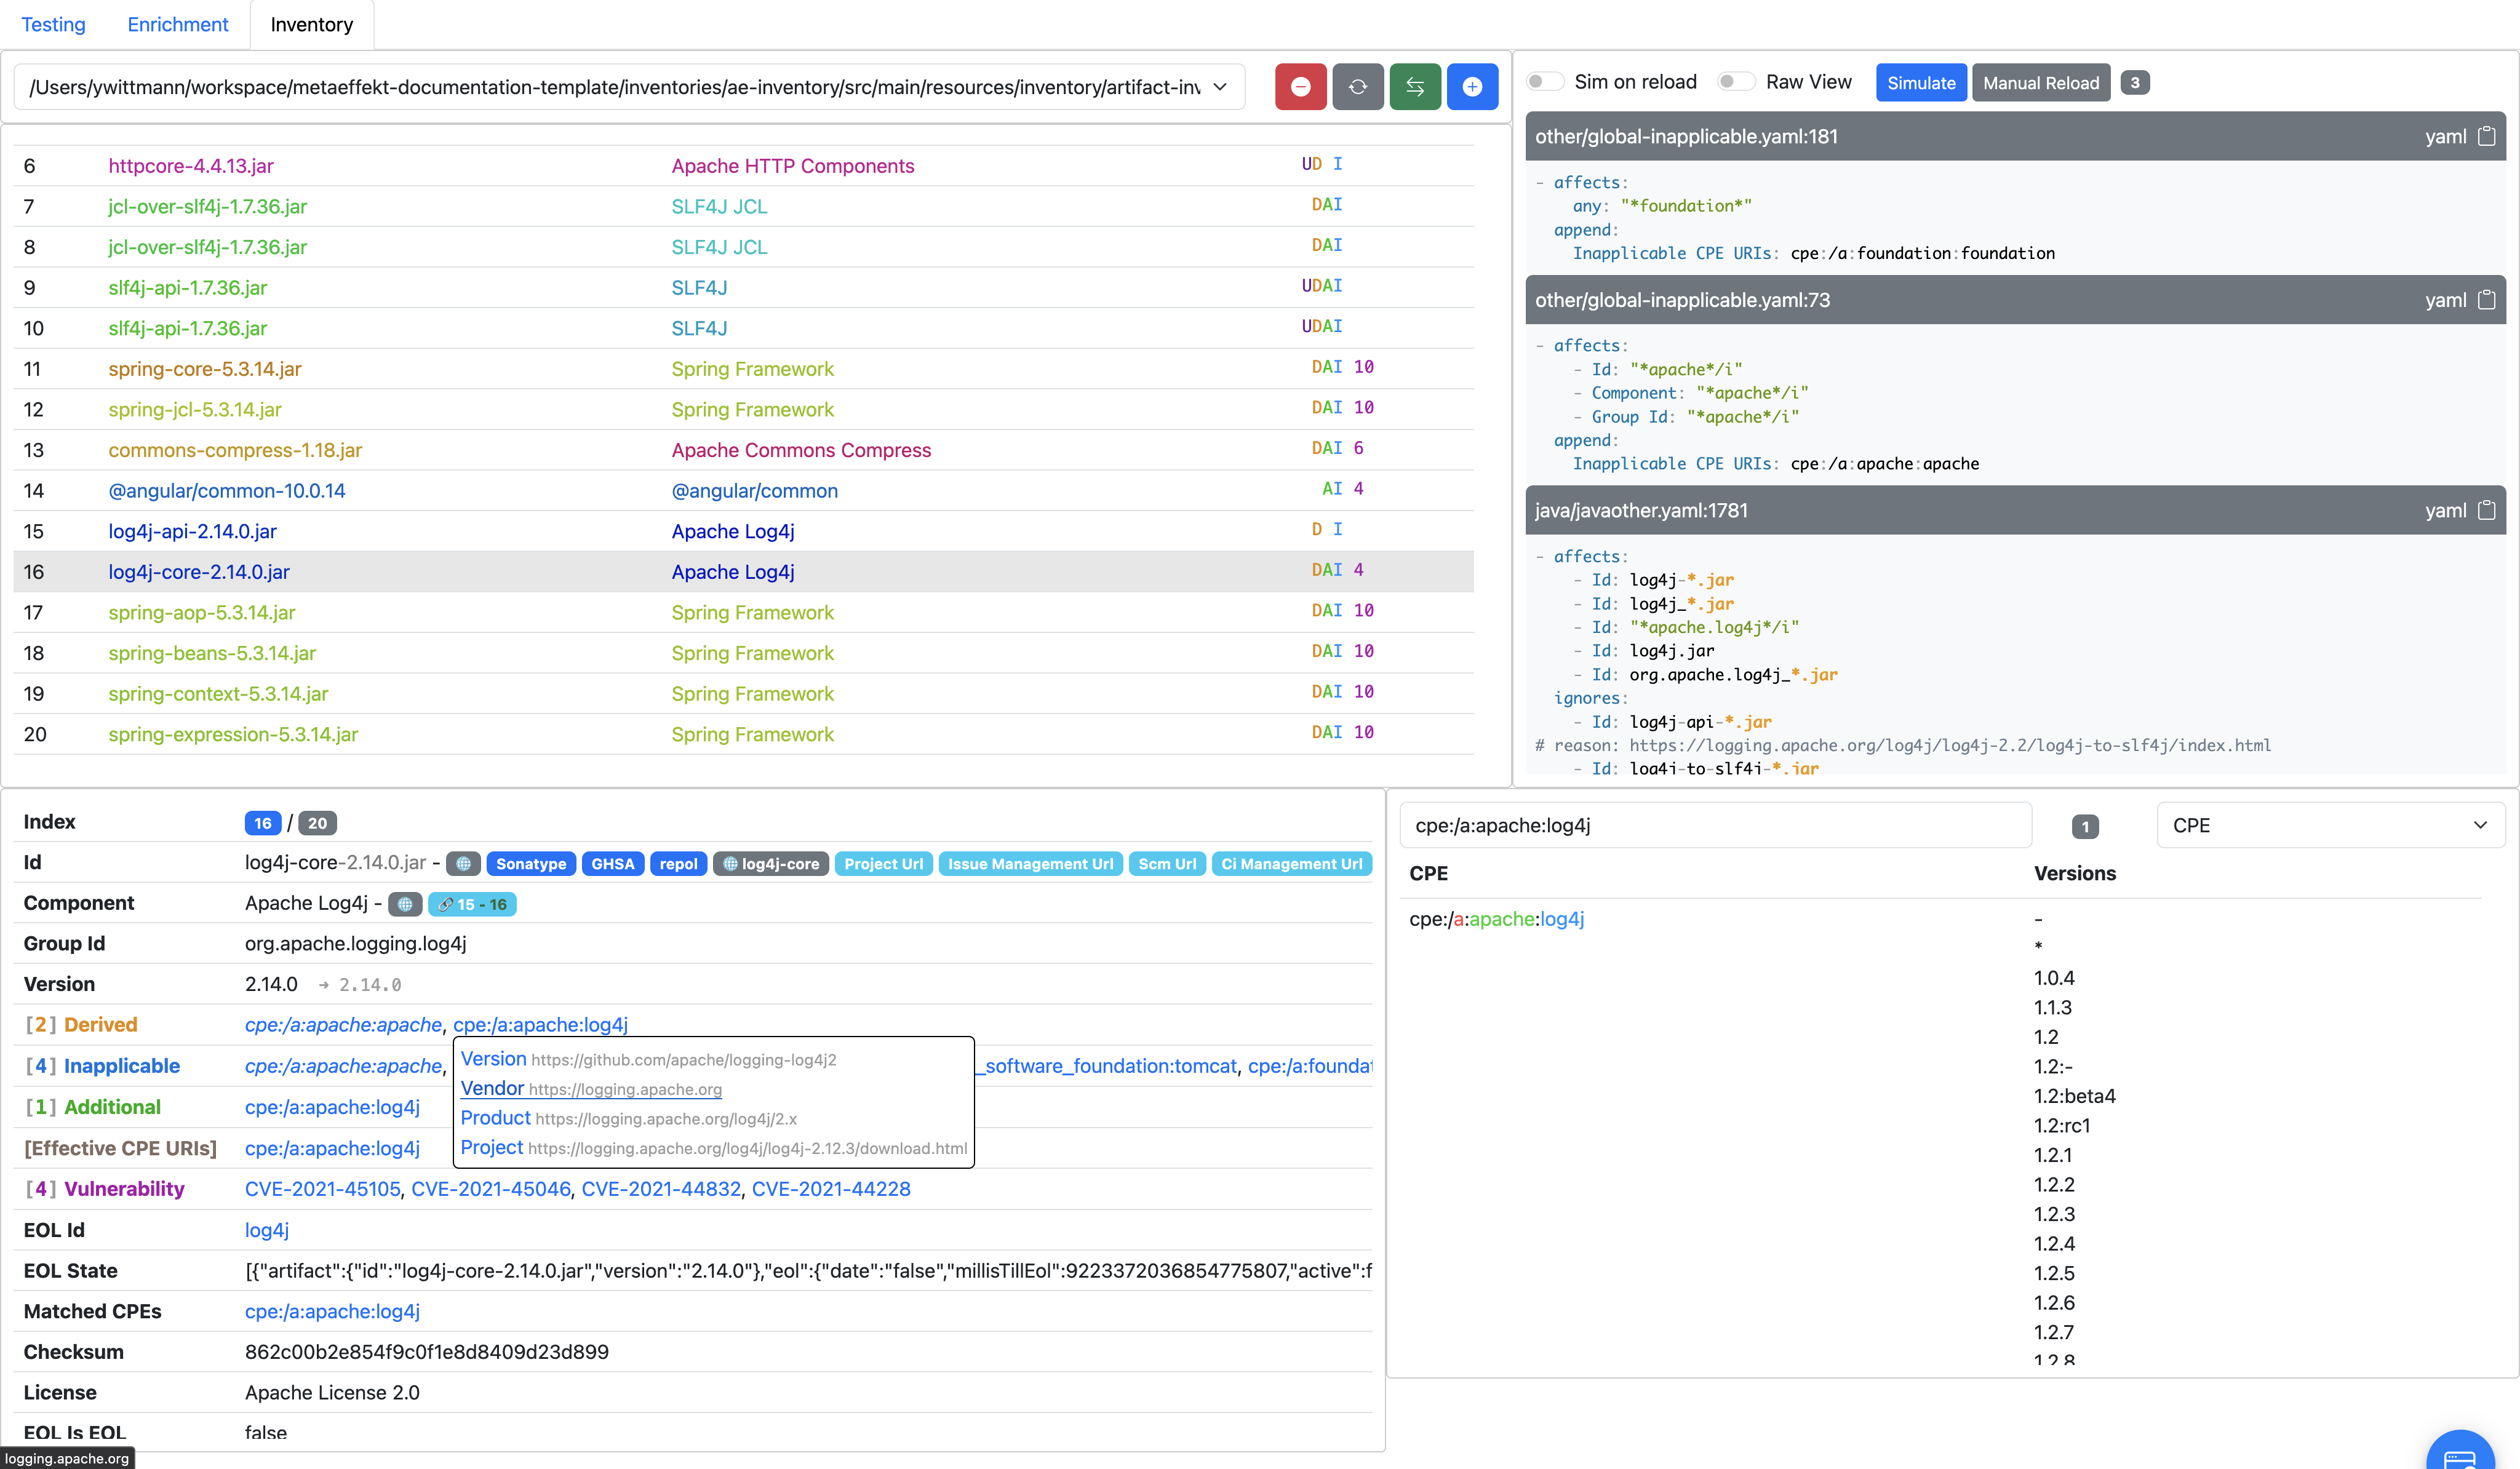
\includegraphics[keepaspectratio,width=1.3\linewidth]{../../images/correlation-utilities-demo}}
    \caption{Das Artefakt \texttt{log4j-core-2.14.0.jar} in den Correlation Utilities}
    \label{fig:correlation-utilities-demo}
\end{figure}

Ein weiteres Widget auf der rechten Seite zeigt, welche Korrelationseinträge auf das aktuelle Artefakt angewendet wurden und erlaubt über eine Integration mit IntelliJ IDEA den direkten Zugriff auf die Korrelationseinträge im Editor und schlägt auf der Basis von einigen bekannten Mustern neue Einträge vor, die mit einem Klick übernommen werden können.
Die Korrelationseinträge werden automatisch bei Änderungen in den Dateien neu geladen und ausgewertet.
Unten rechts kann eine integrierte Abfrageschnittstelle zu den lokalen Datenbanken gefunden werden, über die Abfragen etwa zu \acrshortpl{cpe}, \acrshortpl{cve} oder Produktversionen getätigt werden können.

% TODO: actually perform test, ask Julian
% \smallskip
% Nach einem internen Test hat sich herausgestellt, dass Mitarbeiter mit den Utilities mehr als 2.5-mal so schnell dieselbe Arbeit in höherer Ergebnisqualität durchführen konnten, wie wenn sie dieses Tool nicht verwendet hätten.

\paragraph{Fallunterscheidungen je Artefakt}
Für den allgemeinen Arbeitsablauf mit diesem Tool gibt es pro Artefakt mehrere Fälle, die auftreten können:

\begin{itemize}
    \item Wenn das Artefakt \enquote{Derived CPE URIs} hat, die nicht von einem der weiteren \acrshort{cpe}-Attribute (Additional, Ignores, \ldots) abgedeckt sind, dann bedeutet dies, dass die \acrshortpl{cpe} noch nicht manuell behandelt und geprüft wurden.
    Diese Art von \acrshort{cpe} auf einem Artefakt nennt sich im Tool \enquote{Untouched CPEs}.
    Nachdem sie auf ihre Richtigkeit geprüft wurden, muss die Entscheidung über einen vorhandenen oder neuen Korrelationseintrag in einem der manuellen \acrshort{cpe}-Attribute festgehalten werden.
    Doch nicht nur die automatisch hinzugefügten \acrshort{cpe} müssen untersucht werden, es muss auch nach zusätzlichen \acrshortpl{cpe} im Internet oder den lokalen Datenbanken gesucht werden, um sicherzustellen, dass alle korrekten \acrshort{cpe} gefunden werden.

    \item Wenn das Artefakt nur manuelle \acrshort{cpe}-Attribute gesetzt hat, dann handelt es sich bei diesem Artefakt um ein bereits bekanntes, welches in der Vergangenheit einmal bearbeitet wurde.
    In den meisten Fällen ist hier keine neue Arbeit nötig.
    Manchmal jedoch gibt es Fälle, in denen ein Artefakt seit der letzten Analyse eine neue \acrshort{cpe} zugewiesen bekommen hat, etwas bei dem vorherigen Durchgang übersehen wurde, oder es sich um eine Fehlidentifikation in den Korrelationsdaten handelt und diese fehlerhaft hinzugefügt wurde.
    Je nach Attribut-Kombination sind unterschiedliche Fälle wahrscheinlicher, für welche eine Person mit der Zeit ein Gefühl bekommt.

    \item Wenn das Artefakt überhaupt keine \acrshort{cpe}-Information hat, dann muss manuell nachgeprüft werden, ob es zusätzliche gibt, die diesem Produkt entsprechen.
    Wenn eine oder mehrere passende gefunden werden, wird mit diesen ein neuer Korrelationseintrag angelegt.
\end{itemize}

Vor allem bei einem ersten Durchlauf eines Software-Inventars treten die ersten beiden Fälle häufig auf, aber auch bei erneuten Analysen bekannter Inventare müssen die Artefakte auf ihre Richtigkeit geprüft werden.
